\chapter{Funções de Hash}
\label{cha:hash}

Uma função de hash é uma ferramenta que pega uma sequência de dados de qualquer tamanho e a transforma em uma sequência curta e de tamanho fixo.
Chamaremos de {\em resumo} essa sequência curta, mas que em inglê ela é conhecida como {\em digest} ou {\em checksum}.

Quando estudamos funções de hash em Estrutura de Dados, o objetivo é geralmente otimizar o acesso a uma lista, permitindo que encontremos elementos de maneira muito rápida, em tempoconstante.
Para conseguir isso, tentamos minimizar as colisões, ou seja, tentamos garantir que diferentes entradas não acabem no mesmo local da lista. Isso faz com que a busca seja mais eficiente.

No entanto, em aplicações de criptografia, evitar colisões é ainda mais importante.
Se duas entradas diferentes resultarem no mesmo resumo, isso pode criar vulnerabilidades que adversários podem explorar para comprometer a segurança do sistema.

Uma função de hash criptográfica é uma função $H$ que pega qualquer sequência de bits como entrada e a transforma em uma sequência de bits de tamanho fixo.

Um aspecto fundamental de uma função de hash criptográfica é sua {\em resistência a colisões}.
Isso significa que deve ser extremamente difícil encontrar duas entradas diferentes que resultem na mesma saída.
Para explicar esse conceito, podemos imaginar um jogo onde o objetivo do adversário é encontrar essas duas entradas diferentes.

Aqui está como podemos imaginar esse jogo:
\begin{enumerate}
\item Primeiro, o sistema gera uma semente $s$ usando um algoritmo.
  Essa semente não precisa ser secreta.
    
\item Em seguida, o adversário recebe essa semente $s$.
  A semente serve como um ponto de partida para tentar encontrar duas mensagens que, ao serem processadas pela função de hash, resultem no mesmo resumo.
    
\item O adversário então tenta encontrar uma colisão, ou seja, um par de mensagens, $m$ e $m'$, que tenham o mesmo resumo ($H_s(m) = H_s(m')$).
\end{enumerate}

O sistema é considerado {\em seguro contra colisões} se nenhum adversário eficiente (polinomial) é capaz de encontrar uma colisão com probabilidade considerável.

\begin{center}
\begin{tikzpicture}[node distance=2cm,auto,>=latex]
\tikzset{
  player/.style={draw,shape=rectangle,rounded corners,minimum width=5em,minimum height=5em}
}
\node[player,draw=none] (adversary) {\stickfigure};
\node[player] (system) at (10,0) {$\Pi$};
\draw[->] (9,0) -> node[above]{$s$} (1,0);
\draw[->] (adversary) -> node{$m, m'$} (0,-2);
\end{tikzpicture}
\end{center}

A semente usada na definição da segurança para funções de hash tem um propósito estritamente técnico.
Sem uma semente, um adversário poderia pré-calcular colisões.

Na prática, normalmente usamos funções de hash sem uma semente e as consideramos seguras contra colisões quando isso é validado empiricamente, ou seja, por meio de testes extensivos e análises práticas.

A resistência à colisão é uma das propriedades mais importantes de uma função de hash, e é uma das mais difíceis de alcançar.
Ela garante que seja extremamente difícil encontrar duas entradas diferentes que resultem na mesma saída.
Essa propriedade é mais forte do que outras propriedades que também desejamos em funções de hash, como:
\begin{itemize}
\item[] {\em Resistência contra colisões em alvos específicos}:
  Dado um valor $s$ e uma entrada $m$, nenhum adversário eficiente deve ser capaz de encontrar outra entrada $m'$  tal que $H_s(m) = H_s(m')$ com uma probabilidade significativa.
  Isso significa que, mesmo se alguém souber a saída $H_s(m)$, ele não deve ser capaz de encontrar outro valor que produza o mesmo resultado.
\item[] {\em Resistência contra preimagem}:
  Dado um valor $s$ e uma saída $y$, nenhum adversário eficiente deve ser capaz de encontrar uma entrada $m$ tal que $H_s(m)=y$ com uma probabilidade considerável.
  Isso significa que, mesmo se alguém souber o resultado de uma função de hash, ele não deve ser capaz de descobrir qual entrada gerou aquele resultado.
\end{itemize}


Toda função de hash está vulnerável a ataques do tipo força bruta. Suponha que temos uma função $H_s$, que mapeia qualquer sequência de bits em uma saída de $n$ bits.
Se calcularmos $H_s(m)$ para uma sequência grande de diferentes entradas, eventualmente encontraremos uma colisão.
Isso é garantido pelo princípio da casa dos pombos:
se temos mais itens do que ``caixas'' para colocá-los, pelo menos duas entradas diferentes acabarão na mesma caixa (ou seja, produzirão o mesmo resumo).


Na verdade, se assumirmos que a função de hash se comporta como uma função aleatória, podemos mostrar que a probabilidade de encontrar uma colisão é maior que $50\%$ se testarmos cerca de $\sqrt{n}$ entradas diferentes.
Esse resultado é conhecido como o {\em paradoxo do aniversário}.
Ele é chamado assim porque, por exemplo, em um grupo de 23 pessoas (pense um time de futebol, com titulares, reservas e o técnico), a chance de duas delas terem o mesmo aniversário é maior que $50\%$.
Embora 23 pessoas pareça um número pequeno para essa coincidência, a matemática por trás do paradoxo explica essa alta probabilidade de colisão.

Portanto, se quisermos um sistema de hash que ofereça segurança equivalente a uma função aleatória com uma chave de 128 bits, precisamos usar uma função de hash que produza uma saída de pelo menos 256 bits.

À primeira vista, encontrar uma colisão qualquer pode parecer inofensivo, já que não controlamos quais valores vão colidir.
No entanto, esse ataque pode ser mais perigoso do que parece.

O ataque do aniversariante exige que sejam testadas cerca de $\sqrt{n}$ mensagens diferentes para que a probabilidade de encontrar uma colisão seja grande.
Aqui, $n$ é o número de possíveis valores de hash.
O ponto crucial é que essas mensagens não precisam ser aleatórias.
Podemos gerar mensagens de forma inteligente, utilizando variações controladas, para aumentar nossas chances de sucesso no ataque.


Vamos ilustrar isso com um exemplo.
Suponha que um grupo de alunos estejam tentando forjar uma grande quantidade de variações de uma avaliação de um professor, de forma que todas pareçam legítimas, mas tenham pequenas diferenças, permitindo explorar o ataque do aniversariante.

Considere as seguintes frases:

\begin{quote}
  O projeto foi {\em executado/ realizado/ concluído} com {\em sucesso/ eficiência/ precisão}, e os {\em resultados/ objetivos} foram {\em atingidos/ superados} dentro do {\em prazo/ tempo/ cronograma} previsto.
  O grupo demonstrou {\em dedicação/ comprometimento/ esforço} durante todo as aulas.
\end{quote}

As palavras em itálico podem ser trocadas entre si sem alterar o sentido geral da mensagem.
Com essa abordagem, podemos gerar 324 variações diferentes da frase (3 opções para a primeira substituição, 3 para a segunda, 2 para a terceira, e assim por diante).

Se precisássemos gerar um conjunto de $2^{32}$ mensagens, poderíamos elaborar um texto com pelo menos 32 palavras onde cada uma tem pelo menos um sinônimo, o que nos permitiria criar um número imenso de versões da mesma mensagem, todas com significado equivalente.

\section{Construções}
\label{sec:construcoes}

A maioria das funções de hash que usamos hoje seguem uma estrutura conhecida como {\em Merkle-Damg\aa rd}.
  Essa construção é uma maneira de estender a segurança de uma função de compressão (que processa mensagens de tamanho fixo) para trabalhar com mensagens de qualquer tamanho, mantendo a resistência a colisões \cite{Merkle89,Damgard89}.

Vamos explorar como essa construção funciona, passo a passo.

Imagine que temos uma função de hash $h$ que pode processar apenas blocos de dados de tamanho fixo -- digamos, ela pega uma entrada de $2n$ bits e a comprime para um resumo de $n$ bits.
Esse tipo de função é chamada de {\em função de compressão}.

Vamos agora entender como construímos uma função de hash completa usando essa ideia:

\begin{itemize}
\item Suponha que temos uma mensagem $m$ de tamanho arbitrário.
  Primeiro, dividimos essa mensagem em blocos menores de tamanho $n$ bits.
  Se o tamanho total da mensagem não for um múltiplo exato de $n$, completamos o último bloco com zeros (isso é chamado de {\em padding}).
\item Definimos um valor inicial como um bloco de 0s que será usado para começar o processo de hashing. 
\item Agora, processamos cada bloco da mensagem, um de cada vez.
  Aplicamos a função de compressão $h$ usando o bloco resultado anterior e o bloco atual da mensagem ($z_i = h(z_{i-1}||m_i)$).
\end{itemize}

\begin{center}
\begin{tikzpicture}[node distance=2cm,auto,>=latex]
  \node (IV) at (0,-2)  {$0^n$};
  \node (m1) at (2,0)  {$m_1$};
  \node (h1) at (2,-2)  {$h_s$};
  \node (m2) at (4,0) {$m_2$};
  \node (h2) at (4,-2)  {$h_s$};
  \node at (6,0) {\dots};
  \node at (6,-2) {\dots};
  \node (ml) at (8,0) {$m_{l+1} = L$};
  \node (hl) at (8,-2)  {$h_s$};
  \node (H) at (10,-2)  {$H_s(m)$};
  \draw[->] (IV) -> node[above]{$z_0$}(h1);
  \draw[->] (m1) -> (h1);
  \draw[->] (h1) -> node[above]{$z_1$}(h2);
  \draw[->] (m2) -> (h2);
  \draw[->] (ml) -> (hl);
  \draw[->] (7,-2) -> node[above]{$z_l$}(hl);
  \draw[->] (hl) ->  node[above]{$z_{l+1}$}(H);
\end{tikzpicture}
\end{center}


\begin{theorem}[Merkle-Damg\aa rd]
  Se a função de compressão $h$ para uma mensagem de tamanho fixo é resistente a colisão então a função de hash $H$ construída com o modelo {\em Merkle-Damg\aa rd} para mensagens de tamanho arbitrário é resistente a colisão.
\end{theorem}

\subsection{SHA-1}
\label{sec:sha-1}

O {\em Secure Hash Algorithm 1} (SHA-1) é um algoritmo de hash que pertence à mesma família do MD4.
Ele é projetado para pegar uma entrada de tamanho arbitrário (desde que seja menor que $2^{64}$ bits) e produzir um resumo de 160 bits.

Antes que o SHA-1 possa processar a mensagem, ele precisa prepará-la de uma forma específica. Esse processo envolve algumas etapas importantes:

\begin{itemize}
\item[] {\em Preenchimento (``padding'')}:
  Primeiro, a mensagem original é ``preenchida'' para que seu tamanho final seja um múltiplo de 512 bits.
  Esse preenchimento é feito adicionando uma sequência especial de bits ao final da mensagem.

  A sequência de padding começa com um $1$ seguido por uma série de $0$s e, no final, o tamanho original da mensagem em bits.

  O objetivo é garantir que, após o padding, o tamanho total da mensagem seja um múltiplo de 512 bits.
  Isso é importante porque o SHA-1 processa a mensagem em blocos de 512 bits.
\item[] {\em Divisão da Mensagem em Blocos}:
  Após o padding, a mensagem completa é dividida em blocos de 512 bits cada.
\end{itemize}

Com esses blocos prontos, o SHA-1 pode então aplicar seu algoritmo para processar cada bloco e gerar o resumo final de 160 bits.
Esse resumo é uma representação compacta e segura da mensagem original, útil para garantir a integridade e a autenticidade dos dados em diversas aplicações de segurança.

Na construção Merkle-Damg\aa evrd, a função de hash $h$ desempenha um papel crucial, processando os blocos de dados para gerar o resumo final.
Essa função $h$ consiste em 80 rodadas de cálculos, onde a mensagem é processada em partes para garantir que o resultado final seja seguro e resistente a ataques.

O processo começa com o \textit{message schedule}, que gera 80 strings de 32 bits cada, chamadas $W_0, \dots, W_{79}$, a partir do bloco $x_i$ da mensagem que está sendo processado.
Essas strings são usadas em cada uma das 80 rodadas de processamento da função de hash.

Antes de começar as rodadas, são definidos valores iniciais fixos para cinco variáveis cada uma com 32 bits que podem ser representadas com 8 dígitos hexadecimais: 

\begin{itemize}
  \item[] $A = \texttt{67452301}$
  \item[] $B = \texttt{EFCDAB89}$
  \item[] $C = \texttt{98BADCFE}$
  \item[] $D = \texttt{10325476}$
  \item[] $E = \texttt{C3D2E1F0}$
\end{itemize}

Esses valores serão alterados em cada uma das 80 rodadas para ajudar a processar a mensagem.

Durante as 80 rodadas, os valores $A, B, C, D, E$ são atualizados usando a seguinte fórmula:

\begin{itemize}
\item[] {\em Desloca os Valores:}
  Os valores de $B, C, D, E$ são então deslocados, com $B$ sendo rotacionado 30 bits para a esquerda.

  \begin{displaymath}
    B, C, D, E = A, B_{<<30}, C, D 
  \end{displaymath}

\item[] {\em Atualiza $A$:}
  O novo valor de $A$ é calculado somando o valor de $E$, uma função específica $f_t(B,C,D)$ que depende dos valores de $B, C, D$, uma versão rotacionada de $A$, a string $W_t$ correspondente à rodada, e uma constante $K_t$.

  \begin{displaymath}
    A = E \xor f_t(B,C,D) \xor A_{<<5} \xor W_t \xor K_t
  \end{displaymath}
\end{itemize}

\begin{center}
  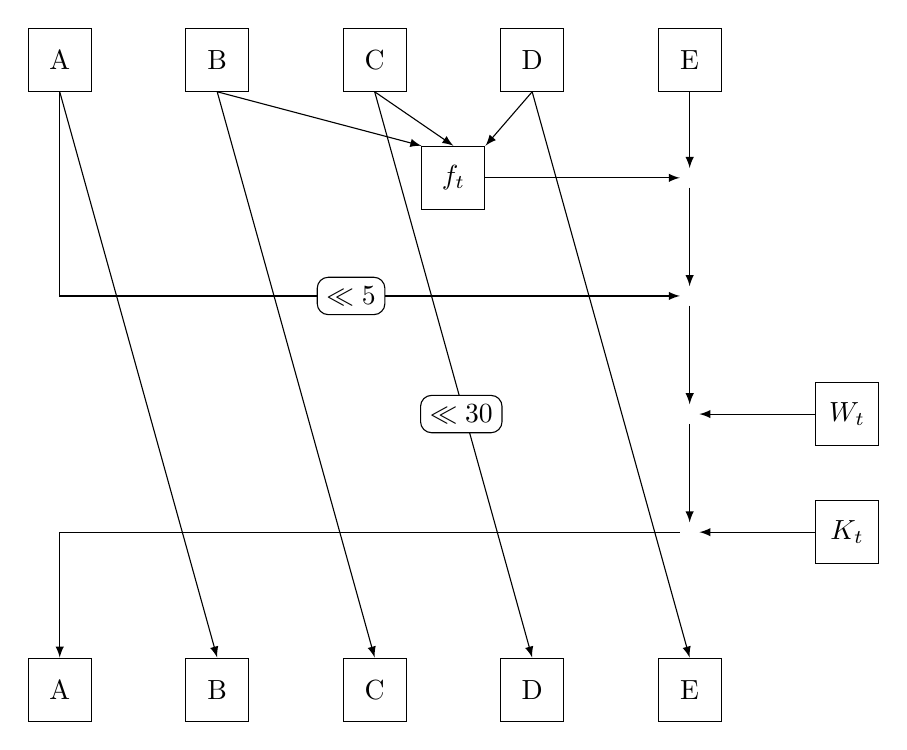
\begin{tikzpicture}
    % Define os vetores
    \node[draw, minimum width=0.8cm, minimum height=0.8cm] (A1) at (0, 0) {A};
    \node[draw, minimum width=0.8cm, minimum height=0.8cm] (B1) at (2, 0) {B};
    \node[draw, minimum width=0.8cm, minimum height=0.8cm] (C1) at (4, 0) {C};
    \node[draw, minimum width=0.8cm, minimum height=0.8cm] (D1) at (6, 0) {D};
    \node[draw, minimum width=0.8cm, minimum height=0.8cm] (E1) at (8, 0) {E};
    
    \node[draw, minimum width=0.8cm, minimum height=0.8cm] (A2) at (0, -8) {A};
    \node[draw, minimum width=0.8cm, minimum height=0.8cm] (B2) at (2, -8) {B};
    \node[draw, minimum width=0.8cm, minimum height=0.8cm] (C2) at (4, -8) {C};
    \node[draw, minimum width=0.8cm, minimum height=0.8cm] (D2) at (6, -8) {D};
    \node[draw, minimum width=0.8cm, minimum height=0.8cm] (E2) at (8, -8) {E};

    % Adiciona setas entre os elementos, do meio da parte inferior ao meio da parte superior
    \draw[-latex] (A1.south) -- (B2.north);
    \draw[-latex] (B1.south) -- (C2.north);
    \draw[-latex] (C1.south) -- (D2.north);
    \draw[-latex] (D1.south) -- (E2.north);

    % Adiciona um nó para a anotação de shift <<30
    \node[draw, fill=white, rounded corners] at (5.1, -4.5) {$\ll 30$};

    % Nós intermediários f_t e XOR_1
    \node[draw, minimum width=0.8cm, minimum height=0.8cm] (ft) at (5, -1.5) {$f_t$};
    \node (XOR1) at (8, -1.5) {\Large $\xor$};

    % Setas de B, C e D para f_t e de f_t para XOR_1
    \draw[-latex] (B1.south) -- (ft.north west);
    \draw[-latex] (C1.south) -- (ft.north);
    \draw[-latex] (D1.south) -- (ft.north east);
    \draw[-latex] (ft.east) -- (XOR1.west);

    \node (XOR2) at (8, -3) {\Large $\xor$};

    % Nós intermediários XOR_3 e W_t com setas
    \node (XOR3) at (8, -4.5) {\Large $\xor$};
    \node[draw, minimum width=0.8cm, minimum height=0.8cm] (Wt) at (10, -4.5) {$W_t$};
    \draw[-latex] (Wt.west) -- (XOR3.east);

    % Nós intermediários XOR_4 e K_t com setas
    \node (XOR4) at (8, -6) {\Large $\xor$};
    \node[draw, minimum width=0.8cm, minimum height=0.8cm] (Kt) at (10, -6) {$K_t$};
    \draw[-latex] (Kt.west) -- (XOR4.east);

    % Conexões finais entre os nós intermediários
    \draw[-latex] (A1.south) -| (0, -3) |- (XOR2.west);

    % Adiciona um nó para a anotação de shift <<5
    \node[draw, fill=white, rounded corners] at (3.7, -3) {$\ll 5$};
    
    \draw[-latex] (E1.south) -- (XOR1.north);
    \draw[-latex] (XOR1.south) -- (XOR2.north);
    \draw[-latex] (XOR2.south) -- (XOR3.north);
    \draw[-latex] (XOR3.south) -- (XOR4.north);

    % Seta final de XOR_4 para A2 com curva
    \draw[-latex] (XOR4.west) -| (0, -6) -| (A2.north);
    
  \end{tikzpicture}
\end{center}

Para adicionar uma camada extra de complexidade e segurança, as constantes $K_t$ e as funções $f_t(B,C,D)$ mudam a cada 20 rodadas:

\begin{enumerate}
\item {\em Rodadas 0-19:}
  \begin{itemize}
  \item[] $K_t := \texttt{5A827999}$
  \item[] $f_t(B,C,D) := (B \land C) \lor (B \land D)$
  \end{itemize}
\item {\em Rodadas 20-39:}
  \begin{itemize}
  \item[] $K_t := \texttt{6ED9EBA1}$
  \item[] $f_t(B,C,D) := B \xor C \xor D$
  \end{itemize}
\item {\em Rodadas 40-59:}
  \begin{itemize}
  \item[] $K_t := \texttt{8F1BBCDC}$
  \item[] $f_t(B,C,D) := (B \land C) \lor (B \land D) \lor (C \land D)$
  \end{itemize}
\item {\em Rodadas 60-79:}
  \begin{itemize}
  \item[] $K_t := \texttt{CA62C1D6}$
  \item[] $f_t(B,C,D) := B \xor C \xor D$
  \end{itemize}
\end{enumerate}

Para cada bloco continuamos o processo partindo dos valores de $A, B, C, D$ e $E$ com os quais termiamos no bloco anterior.
Ao final do processo, o valor do hash é formado pela concatenação dos valores contidos nessas variáveis.

Em fevereiro de 2017, um grupo de pesquisadores da Google, em parceria com uma universidade holandesa, anunciou ter conseguido realizar um ataque prático ao algoritmo de hash SHA-1, demonstrando que é possível encontrar colisões -- ou seja, duas entradas diferentes que produzem o mesmo hash.

Os pesquisadores estimaram que, em um ataque de força bruta, levaria cerca de um ano utilizando aproximadamente 12 milhões de processadores gráficos (GPUs) para encontrar uma colisão no SHA-1.
No entanto, ao explorar vulnerabilidades específicas do SHA-1, eles conseguiram reduzir drasticamente esse número, realizando o ataque com apenas 110 processadores\footnote{https://security.googleblog.com/2017/02/announcing-first-sha1-collision.html}.

Para provar a eficácia do ataque, eles criaram dois documentos PDF diferentes.
Cada documento continha um infográfico explicando o ataque, mas com cores diferentes.
O impressionante é que, apesar de serem documentos distintos, ambos produziam exatamente o mesmo hash quando processados pelo SHA-1.

Este ataque prático ao SHA-1 foi um sinal claro de que o algoritmo não é mais seguro para uso em aplicações que exigem alta segurança.
A recomendação atual é utilizar algoritmos de hash mais robustos e confiáveis, como o SHA-256 ou o SHA-3, que oferecem uma resistência muito maior contra colisões e outros tipos de ataques.

\section{Aplicações}
\label{sec:aplicacoes}

As funções de hash são ferramentas essenciais em protocolos de segurança, com diversas aplicações que garantem a integridade e a segurança dos dados.
Nesta seção, vamos explorar quatro aplicações distintas dessas funções:

\begin{itemize}
\item[] {\em Código de Autenticação de Mensagem baseado em Hash (HMAC)}:
  Um sistema de autenticação amplamente utilizado, que usa funções de hash para assegurar que uma mensagem não foi alterada e que sua origem é autêntica.
  HMAC é especialmente popular em protocolos de comunicação segura, como SSL/TLS.

\item[] {\em Derivação de Subchaves a Partir de Outras Chaves}:
  Funções de hash podem ser usadas para gerar subchaves seguras a partir de uma chave principal.
  Isso é útil em sistemas onde uma única chave mestre precisa ser subdividida em várias chaves menores para diferentes finalidades, mantendo a segurança geral do sistema.

\item[] {\em Derivação de Chaves a Partir de Senhas}:
  Em muitos sistemas, é necessário converter uma senha em uma chave criptográfica.
  As funções de hash desempenham um papel crucial nesse processo, transformando a senha em uma chave segura que pode ser usada para criptografia, garantindo proteção contra ataques como força bruta.
\end{itemize}
  
Essas aplicações demonstram a versatilidade e a importância das funções de hash em várias áreas da segurança da informação.
Vamos examinar cada uma delas em mais detalhes.

\subsection{HMAC}
\label{sec:hmac}

No capítulo anterior, discutimos como criar um sistema de autenticação para mensagens de tamanho arbitrário usando um esquema semelhante ao modo CBC.
Agora, vamos explorar uma abordagem alternativa chamada {\em Hash-and-MAC}.

Em vez de autenticar diretamente a mensagem de tamanho arbitrário, a ideia por trás do Hash-and-MAC é primeiro comprimir a mensagem em um valor de tamanho fixo, o resumo, usando uma função de hash.
Em seguida, aplicamos um sistema de autenticação para esse resumo, como se fosse uma mensagem de tamanho fixo.
Esse método é muito eficaz e é amplamente utilizado em protocolos de segurança.

Considere que temos um sistema de autenticação para mensagens de tamanho fixo $\Pi_M$ e uma função de hash $H$ resistente contra colisão que produz um resumo de tamanho $n$.

O sistema \textit{Hash-and-MAC} $\Pi$ para mensagens de tamanho arbitrário é construído da seguinte maneira:

\begin{itemize}
\item[] {\em Geração de Chaves}:
  Gera uma chave composta por duas partes: $k_M$, a chave usada pelo sistema de autenticação, e $s$, a chave usada pela função de hash. 
  
\item[] {\em Geração do CAM}:
  Para autenticar uma mensagem $m$ de tamanho arbitrário, primeiro calculamos o \textit{resumo} $H_s(m)$ usando a função de hash.
  Em seguida, aplicamos o sistema de autenticação de tamanho fixo $Mac_M$ ao \textit{resumo} para gerar o código de autenticação ($Mac(k, m) := Mac_M(k_M, H_s(m))$).
  
\item[] {\em Verificação}:
  Verificamos a mensagem exatamente da mesma forma como nos modos que já apresentamos.
\end{itemize}


\begin{theorem}
  Se $\Pi_M$ é um sistema de autenticação seguro contra falsificação e $H$ é um hash resistente a colisão então a construção acima é segura contra falsificação.
\end{theorem}
\begin{proof}
A ideia central da prova é a seguinte: 
Imagine um adversário que tenta quebrar a segurança do sistema, consultando os códigos de autenticação (tags) de uma série de mensagens $Q$.
Agora, vamos supor que, de alguma forma, o adversário consiga gerar um código válido para uma nova mensagem $m$ que não estava na lista $Q$.

Se isso fosse possível, teríamos dois cenários:
\begin{enumerate}
\item Suponha que existe uma mensagem $m'$ em $Q$ tal $H_s(m') = H_s(m)$.
  Isso contraria a segurança contra colisões de $H$.
\item Se não há colisão, então o adversário teria conseguido gerar um código de autenticação válido para uma nova mensagem, a partir do resumo $H_s(m)$, que tem um tamanho fixo.
  Isso contradiria a hipótese de que o sistema de autenticação $\Pi_M$  é seguro contra falsificação.
\end{enumerate}

\end{proof}

O HMAC é um sistema de autenticação baseado no paradigma Hash-and-MAC, sendo um dos mais amplamente utilizados em protocolos de segurança.
Ele funciona aplicando uma função de hash duas vezes sobre a combinação de uma chave secreta com os dados, utilizando duas constantes diferentes, chamadas {\tt ipad} e {\tt opad}.
Exemplos de sua aplicação incluem os protocolos TLS/SSL, que garantem a integridade e autenticidade de dados transmitidos em conexões seguras, como o HTTPS, o IPsec, que autentica e protege pacotes de dados em redes IP, como em VPNs, e o SSH, que assegura a integridade dos dados durante transferências seguras.

Vamos entender como o HMAC funciona:

\begin{itemize}
\item Primeiro, combinamos a chave $k$ com a constante {\tt ipad} usando a operação XOR.
\item Em seguida, aplicamos a função de hash $H_s$ ao resultado dessa combinação junto com a mensagem $m$.
\item Depois disso, combinamos a chave $k$ com a constante {\tt opad} (também usando XOR).
\item Finalmente, aplicamos a função de hash $H_s$ a essa nova combinação junto com o resultado do primeiro hash.
\end{itemize}

\begin{displaymath}
Mac(k, m) := H_s((k \xor \textrm{\tt opad}) || H_s(k \xor \textrm{\tt ipad}) || m)
\end{displaymath}

O processo de verificação é identico aos demais que vimos anteriormente.

\subsection{Funções de Derivação de Chaves}
\label{sec:kdf}

Uma {\em função de derivação de chaves} (FDC) é uma ferramenta essencial em criptografia, projetada para gerar uma chave segura a partir de um material que contém uma quantidade significativa de entropia, chamado de {\em material da chave}.

Existem duas situações comuns em que uma FDC é útil:

\begin{itemize}
\item[] {\em Preparação de Material Criptográfico}:
  Às vezes, o material que você tem (como uma senha) não está suficientemente seguro ou preparado para ser usado diretamente como uma chave criptográfica.
  Nesse caso, a FDC ajuda a transformar esse material em uma chave segura.

\item[] {\em Derivação de Subchaves}:
  Quando você tem uma chave inicial e precisa gerar várias subchaves diferentes a partir dela, a FDC pode ser usada para criar essas subchaves de forma segura.
\end{itemize}

Formalmente, uma FDC recebe como entrada:

\begin{itemize}
\item[] O material da chave $\delta$, que é o material base para derivar a chave.
\item[] O tamanho $l$ da chave que queremos produzir.
\item[] Opcionalmente, um valor chamado salt ($r$), que é uma chave pública adicional usada para garantir que a saída seja única, mesmo se o mesmo key material for usado novamente.
\item[] Um valor contextual $c$, que pode ser utilizado para fornecer informações adicionais sobre o contexto em que a chave será usada.
\end{itemize}

Uma FDC segura deve usar esses valores para produzir uma sequência {\em pseudoaleatória} de bits do tamanho desejado $l$.

Uma FDC típica funciona em duas etapas:
\begin{itemize}
\item[] {\em Extração}:
  Nesta etapa, a FDC recebe o $\delta$ e, opcionalmente, um valor público conhecido como salt.
  O objetivo é processar esses valores para produzir uma sequência de bits pseudoaleatória de tamanho fixo.
\item[] {\em Expansão}:
  Na segunda etapa, a sequência de bits produzida na fase de extração é expandida para o tamanho final desejado $l$.
  Isso garante que a chave gerada seja adequada para o uso pretendido.
\end{itemize}

Essas duas etapas juntas garantem que a chave derivada seja segura e adequada para criptografia, seja para substituir uma senha insegura por uma chave robusta ou para gerar subchaves seguras a partir de uma chave inicial.

Uma implementação popular do modelo de função de derivação de chaves (FDC) é o {\em FDC baseada no HMAC} (HKDF) \cite{Krawczyk10}.
Vamos ver como ele funciona:

{\em Passo 1: Extração}

Na fase de extração, o HKDF usa o HMAC para processar o material de chave $\delta$ junto com um valor opcional chamado {\em salt} ($r$).
O resultado dessa operação é uma chave pseudoaleatória (CPA):

\begin{displaymath}
\text{CPA} := \text{HMAC}(r, \delta)
\end{displaymath}

{\em Passo 2: Expansão}

Na fase de expansão, o HKDF usa a CPA gerada na fase de extração para produzir a chave final de tamanho $l$ desejado.
Isso é feito em várias etapas, concatenando blocos de saída $K(1), K(2), \dots$ até que o tamanho total $l$ seja atingido:

\begin{displaymath}
\text{HKDF}(r, \delta, c, l) := K(1) || K(2) \dots || K(t)
\end{displaymath}

Aqui está como cada bloco $K(i)$ é gerado:

\begin{itemize}
    \item {\em Primeiro Bloco}:
    \begin{displaymath}
      K(1) := \text{HMAC}(\text{PRK}, c || 0)
    \end{displaymath}

    Onde $c$ é um valor contextual opcional e 0 é um byte adicional para garantir que o primeiro bloco seja único.

    \item {\em Blocos Subsequentes}:
    \begin{displaymath}
    K(i + 1) := \text{HMAC}(\text{PRK}, K(i) || c || i)
    \end{displaymath}
    
    Onde $K(i)$ é o bloco anterior, $c$ é o valor contextual, e $i$ é um contador que garante que cada bloco gerado seja diferente.
\end{itemize}

A concatenação de todos os blocos $K(1), K(2), \dots$ forma a chave final gerada pelo HKDF.

O HKDF garante que a chave derivada seja segura, mesmo quando o \textit{material da chave} original não é ideal, e é altamente flexível, permitindo a derivação de chaves de qualquer tamanho desejado.
Além disso, o uso do HMAC como base garante que o HKDF herde as propriedades de segurança bem estabelecidas dessa construção.


Quando o \textit{material da chave} $\delta$ é uma senha fornecida por um usuário, enfrentamos um desafio adicional.
Normalmente, as senhas têm uma {\em entropia baixa}, ou seja, elas não são suficientemente aleatórias.
Isso as torna vulneráveis a ataques conhecidos como {\em ataques de dicionário}, onde um adversário tenta adivinhar a senha testando várias combinações comuns.

Para mitigar esse problema, podemos usar uma {\em função de derivação de chaves lenta}.
Isso significa que a função é projetada para ser intencionalmente demorada, dificultando o trabalho de um adversário que tenta executar um grande número de tentativas para adivinhar a senha.

Um tipo popular de função de derivação de chaves baseada em senha é o {\em Password-Based Key Derivation Function 2} (PBKDF2).

O PBKDF2 recebe como parâmetros:
\begin{itemize}
    \item[] {\em Salt $r$}: Um valor aleatório que é adicionado à senha para garantir que senhas iguais resultem em chaves diferentes.
    \item[] {\em Tamanho $l$}: O tamanho da chave final que queremos gerar.
    \item[] {\em Senha $\delta$}: A senha fornecida pelo usuário.
    \item[] {\em Número de ciclos $n$}: Um valor que especifica quantas vezes a função de hash será aplicada, tornando o processo mais lento e seguro.
\end{itemize}

O PBKDF2 gera a chave final em várias etapas:

\begin{displaymath}
  \text{PBKDF2}(r, \delta, c, n, l) := K(1) || K(2) || \dots || K(t)
\end{displaymath}

Aqui está como cada bloco $K(i)$ é calculado:

\begin{itemize}
    \item[] {\em Cálculo do Bloco $K(i)$}:
    \begin{displaymath}
    K(i) := U_0^i \oplus U_1^i \oplus \dots \oplus U_n^i
    \end{displaymath}
    
    Onde cada $U_j^i$ é uma sequência de bits gerada em várias iterações.

    \item[] {\em Primeira Iteração}:
    \begin{displaymath}
    U_0^i := H(\delta || r || i)
    \end{displaymath}
    Nesta etapa, a função de hash $H$ é aplicada à combinação da senha $\delta$, do salt $r$, e do número do bloco $i$.

    \item[] {\em Iterações Subsequentes}:
    \begin{displaymath}
    U_j^i := H(\delta || U_{j-1}^i)
    \end{displaymath}
    Cada iteração subsequente aplica a função de hash $H$ à combinação da senha $\delta$ e do resultado da iteração anterior $U_{j-1}^i$.
\end{itemize}

Cada bloco $K(i)$ é gerado após $n$ iterações da função de hash, tornando o processo computacionalmente caro e, portanto, mais seguro contra ataques.

O uso do {\em salt} impede que um adversário prepare um dicionário de senhas e hashes comuns antes do ataque (preprocessamento).
Isso significa que, mesmo que duas pessoas usem a mesma senha, elas terão hashes diferentes.

O valor de $n$ deve ser suficientemente grande para garantir que a derivação da chave seja lenta, dificultando a criação de um ataque por dicionário, mesmo que o adversário tenha acesso ao hash gerado.
Para um usuário legítimo, o processo de verificação da chave geralmente ocorre poucas vezes, e um atraso de alguns décimos de segundo por tentativa não compromete significativamente a usabilidade do sistema.
No entanto, para um adversário que tenta testar milhões de combinações de chaves, o tempo adicional por iteração torna o ataque impraticável.
Isso porque o tempo necessário para testar cada chave será centenas, ou até milhares de vezes mais lento em comparação com a simples aplicação de uma função de hash única.

O PBKDF2, ao incorporar essas características, oferece uma proteção robusta contra ataques de dicionário e é amplamente utilizado em sistemas de autenticação e armazenamento de senhas.

\section{Exercícios}
\label{sec:exercicios}

\begin{exercicio}
  Mostre que resistência contra colisões garante a resistência contra preimagem.
\end{exercicio}

\begin{exercicio}
  Mostre que o seguinte sistema não é seguro contra falsificação considerando que o sistema de hash foi construído a partir do paradigma de Merkle-Damgard:
\begin{itemize}
\item $Gen(1^n) := k \leftarrow \{0,1\}^n$
\item $Mac(k,m) := H(k||m)$
\item $Ver(k,m,t) := \left\{
    \begin{array}{lcl}
      1 & \textrm{se} & Mac(k,m) = t\\
      0 & \textrm{c.c.} &\\
    \end{array}
    \right.$
\end{itemize}
\end{exercicio}

\begin{exercicio}
  {\em Prova de trabalho} é uma medida para garantir que um determinado usuário tenha que executar uma certa quantidade de processamento durante a excecução de um protocolo.
  Essa ideia é usada na mineração de bitcoins e para evitar spams.
  No segundo caso, brevemente, a ideia é exigir uma quantidade mínima de processamento para um cliente que envie um email.
  Essa quantidade é desprezível para quem manda algumas dezenas de emails por dia, mas é muito cara para quem deseja mandar milhões de spams.

  Uma forma de prova de trabalho é entregar para o cliente a saída de um hash e pedir para que ele compute uma entrada que produza aquela saída.
  Agumente que, se a função de hash escolhida é segura contra colisão, o melhor que o cliente pode fazer é gerar valores aleatórios de entrada até encontrar um cuja a saída coincida com o resultado esperado.
\end{exercicio}

\begin{exercicio}
  Explique com suas palavras a definição de segurança de hashes.
  Por que o SHA-1 não é mais considera segura?
\end{exercicio}
